\documentclass[11pt]{article}

\usepackage[letterpaper,margin=1in]{geometry}
\usepackage[utf8]{inputenc}
\usepackage[T1]{fontenc}
\usepackage{lmodern}
\usepackage{microtype}
\usepackage{graphicx}
\usepackage{booktabs}
\usepackage{tabularx}
\usepackage{longtable}
\usepackage{multirow}
\usepackage{amsmath,amssymb}
\usepackage{enumitem}
\usepackage{float}
\usepackage{placeins}
\usepackage{tikz}
\usetikzlibrary{arrows.meta,positioning,fit}
\usepackage[numbers,sort&compress]{natbib}
\usepackage[colorlinks=true,allcolors=blue]{hyperref}
\setlength{\emergencystretch}{2em}

\graphicspath{{figures/}}
\newcommand{\sepa}{\textsc{SepAware}}
\newcommand{\dacpf}{\textsc{DACPF}}
\newcommand{\tstr}{\textsc{TSTR}}
\newcommand{\trtr}{\textsc{TRTR}}
\newcommand{\ra}{Real$\rightarrow$Real}
\newcommand{\sr}{Synthetic$\rightarrow$Real}
\newcommand{\rsr}{Real+Synthetic$\rightarrow$Real}
\newcommand{\NA}{--}

\newcommand{\review}[1]{{\textbf{\color{red}{#1}}}}
\newcommand{\alex}[1]{{\color{red}[Alex: #1]}}



\title{Improving Rare-Outcome Prediction With Separability-Aware Synthetic Health Data: An Initial Two-Dataset Validation Study}
\author{Oluwatoyin Joy Omole$^{1}$\\
\small $^{1}$Graduate Program in Computer Science, Universidade Federal de Minas Gerais, Belo Horizonte, Brazil\\
\small Author list, degrees, ORCIDs, and corresponding-author details to be confirmed}
\date{}

\begin{document}
\maketitle

\begin{abstract}
\textbf{Background:} Synthetic data are often used to address rare outcomes by increasing minority-class sample size, but additional records may not improve prediction when classes overlap or when generation fails to preserve useful class-conditional structure.

\textbf{Objective:} This study asks when controlling class separability improves the held-out-real utility of synthetic health data beyond class-frequency correction and whether utility gains are accompanied by loss of minority coverage.

\textbf{Methods:} We developed \sepa{}, a post-generation mechanism that selects records from an oversized candidate pool using realism and label-consistent geometric evidence while preserving a prespecified class count. Initial validation used a 5000-record sample of Brazil's Vigitel obesity survey and a 334-record COVID-19 hospital-mortality cohort. Completed analyses include leakage-controlled 5-fold synthetic-to-real evaluation and a blocked $2\times2$ factorial experiment separating separability and anchor pressures. A strengthened augmentation analysis compares real-only training, random sampling, SMOTE, class weighting, conditional tabular generative adversarial networks, tabular variational autoencoders, and their \sepa{}-selected variants. Evaluation includes discrimination, minority-specific performance, calibration, class-conditional coverage, and empirical privacy-risk proxies. A controlled simulation independently varies prevalence and overlap.

\textbf{Results:} In the synthetic-to-real experiment, Vigitel Macro-F1 increased from 0.459 with standard conditional tabular generative adversarial network data to 0.583 with \sepa{}. Separability accounted for 96.00\% of treatment-plus-error variation in the Vigitel factorial analysis ($P<.001$). COVID-19 results were less stable: standard generation achieved 0.463 and the fixed balanced \sepa{} setting achieved 0.549 with wider uncertainty; separability accounted for 5.13\% of variation and residual error for 81.53\%. Across three repeated five-fold partitions in the strengthened augmentation analysis, \sepa{} improved mean AUPRC over standard CTGAN by 0.015 on COVID-19 and 0.013 on Vigitel, but did not improve TVAE. Simple resampling or class weighting matched or exceeded generator-based approaches on most dataset--metric combinations. \sepa{} CTGAN improved nearest-minority coverage while reducing minority diversity. Controlled SepAware-SMOTE gains were small and its overlap and prevalence interactions were not significant.

\textbf{Conclusions:} Initial evidence indicates that class-boundary control is distinct from class balancing and can materially improve synthetic-to-real transfer in some settings. The contrasting datasets also show why SepAware should not be treated as universally beneficial: apparent gains must be tested against uncertainty, calibration, minority coverage, and the possibility that selection merely removes difficult but valid cases.
\end{abstract}

\noindent\textbf{Keywords:} synthetic health data; tabular data; class imbalance; class overlap; rare outcomes; data augmentation; privacy; calibration

\section{Introduction}
\label{sec:introduction}

Health datasets combine sensitive information, mixed numerical and categorical variables, missingness, and outcomes that are often uncommon but clinically consequential \alex{It is necessary to add some references.}. Synthetic tabular data may support model development and collaboration when real records are scarce or difficult to share \alex{It is necessary to add some references.}. Generation, however, does not guarantee privacy or downstream usefulness \citep{goncalves2020,hernandez2023,kaabachi2025}. A generator can preserve aggregate distributions while weakening the class-conditional structure required to recognize a rare outcome \alex{It is necessary to add some references.}. It can also increase apparent predictive performance by exaggerating relationships or selecting unusually easy cases \alex{It is necessary to add some references.}.

Rare-outcome learning is commonly framed as a class-imbalance problem. Random sampling, SMOTE, class weighting, and conditional generation can increase the influence or number of minority observations, but additional records do not necessarily add information \alex{It is necessary to add some references.}. The limiting factor may instead be class overlap \alex{It is necessary to add some references.}: valid positive and negative observations can occupy similar regions of feature space. Class prevalence and class overlap are therefore different properties. Correcting the former does not necessarily repair the latter \alex{It is necessary to add some references.}.

\alex{Here, I think that is necessary to emphasize the literature gap and after to explicitly to define the main goal of work before to describe what will be made/methodology! Also, it is important to explicitly to define the main goal for the research questions are well defined.}

This distinction emerged from our qualification experiments. Conventional rebalancing, unconstrained CTGAN augmentation, and domain-guided candidate filtering produced limited or classifier-dependent gains \alex{It is necessary to add some references.}. Nearest-neighbour and explainability analyses suggested that weak or unstable class geometry remained after augmentation \alex{It is necessary to add some references.}. We therefore developed \sepa{}, a post-generation selection mechanism that draws an oversized candidate pool and ranks records using proximity to the real training manifold and label-consistent geometric evidence. Selection retains a prespecified class count, allowing separability pressure to be studied without attributing every change to class ratio.

The central question is not whether \sepa{} wins on every dataset. It is when control of class separability improves rare-outcome prediction, why the effect differs between datasets, and whether an improvement merely reflects removal of difficult but legitimate minority cases. The contrast already observed between Vigitel obesity and COVID-19 hospital mortality \alex{It is need to put a referente!} provides a useful initial test. Vigitel shows a large and stable synthetic-to-real gain under separability pressure, whereas the COVID-19 effect is smaller relative to fold variation. We treat this contrast as a boundary-condition signal rather than a result to conceal.

\subsection{Research questions}

We investigate three questions \alex{we need to change ``questions'' to ``Research Questions (\textbf{RQ})''! To put the acronym ``\textbf{RQ}:'' before each question and remove the numbers:

- \textbf{RQ1}: Is class frequency correction sufficient, or does class overlap limit the utility of synthetic augmentation?

- \textbf{RQ2}: Does ...

- \textbf{RQ3}: When...}:
\begin{enumerate}[leftmargin=*]
\item Is class frequency correction sufficient, or does class overlap limit the utility of synthetic augmentation? \alex{Here, ``class frequency'' is related to the imbalance-class problem? If so, wouldn't it be better to use the expression ``imbalance class correction'' instead of ``class frequency correction''? Is ``imbalance correction'' at level of data or algorithm? It should be clearer here...}
\item Does separability-aware selection improve rare-outcome prediction beyond random sampling, SMOTE, class weighting, and unconstrained generation?
\item When performance improves, is the gain accompanied by acceptable calibration, minority coverage and diversity, and empirical privacy risk?
\end{enumerate}

The first completed experiment tests mechanism in the synthetic-to-real regime. A leakage-controlled fixed-setting comparison is followed by a blocked $2\times2$ factorial analysis that separates separability and anchor pressures. The strengthened experiment evaluates practical augmentation using real-only training, conventional imbalance methods, CTGAN, TVAE, and \sepa{} variants on shared held-out real folds. It expands evaluation from Macro-F1 to AUPRC, minority-specific measures, AUROC, balanced accuracy, Brier score, calibration parameters, minority coverage and diversity, and privacy-risk proxies.

\alex{Maybe we could describe the main results before we discuss the contributions, this can substantiate and increase the value of contributions! However, the description of results should be more objective.}

\subsection{Contributions}

This initial two-dataset study makes four contributions:
\begin{enumerate}[leftmargin=*]
\item It frames class overlap as a distinct target from class imbalance and global fidelity in synthetic health-data augmentation;
\item It introduces a transparent post-generation selection mechanism whose effect can be separated from generator fitting and class-count correction;
\item It uses a factorial experiment to attribute the strong Vigitel synthetic-to-real change to separability pressure while reporting the COVID-19 null attribution with equal emphasis; \alex{I have a question here, previously, the text states that will use factorial experiments to distinguish ``separability and anchor pressures'', so, what is ``separability pressures''? Are there how much concepts in this expression?}
\item It tests the central rival explanation -- that separability improves prediction by deleting difficult cases -- through minority coverage, diversity, boundary, calibration, and privacy analyses in a strengthened augmentation protocol.
\end{enumerate}

Because only two health datasets are presently available, we describe this work as initial validation. The experimental and manuscript structure is designed for additional datasets, but no claim of broad clinical generalization is made from the current evidence.

\alex{It is important to put a paragraph that describes the structure of paper, this help the reader to understand and give a general view of work.}
\section{Related Work}
\label{sec:related-work}

\alex{Here, the strategy that can works is to introduce and explain the general context to thematic of each section, the existing methods and models and their respective advantages, at end emphasize the literature gap and to discuss how this work fill these gaps.}

\subsection{Synthetic Tabular Health Data}

Synthetic microdata predate deep learning \alex{What is the relationship between microdata with tabular data? I think that lacks an introduction for tabular health-data, because the title of section is about this, but here have no descriptions or concepts for tabular data. Also, the most important is to emphasize that the models mentioned here are related to synthetic tabular data! An objective phrase at the beginning can solve this easily.}. Multiple imputation and probabilistic graphical models generate records from estimated conditional distributions and remain attractive because their assumptions can be inspected \citep{raghunathan2003}. Copulas provide efficient dependence modelling but can struggle when discrete, continuous, multimodal, and rare-event variables interact nonlinearly \citep{wang2021}.

Generative adversarial networks formulate generation as an adversarial game \citep{goodfellow2014}. MedGAN adapted this idea to high-dimensional discrete patient records \citep{choi2017}, and CTGAN addressed mixed-type tables through mode-specific normalization, conditional vectors, and training-by-sampling \citep{xu2019}. Variational autoencoders optimize a likelihood-related lower bound \citep{kingma2014}; TVAE was evaluated alongside CTGAN in the same tabular-synthesis framework \citep{xu2019}. More recently, TabDDPM applied separate diffusion processes to numerical and categorical attributes and outperformed several GAN and VAE baselines \alex{I think that ``extensions'' is better than ``baselines'' here...} on general tabular benchmarks \citep{kotelnikov2023}. The present strengthened analysis uses CTGAN and TVAE to test whether separability-aware selection transfers across generator families; diffusion remains an important future comparator rather than an assumed performance ceiling.

\alex{Here we need to emphasize why your work complement or is better than those ones mentioned here! So, give a little bit more of details (in a objective way)...}

\subsection{Evaluation beyond Aggregate Resemblance}

Health-synthesis studies repeatedly conclude that no single metric establishes usefulness or safety and that evaluation should jointly cover resemblance, downstream utility, and privacy \citep{goncalves2020,hernandez2023,pezoulas2024}. Recent comparisons report dataset- and metric-dependent rankings and a persistent fidelity/utility--privacy trade-off \citep{hernandez2025,nanevski2026}. A review of structured synthetic electronic health records also documents continuing problems with rare events, reproducibility, and privacy evaluation \citep{ghosheh2024}.

Univariate fidelity measures whether synthetic columns resemble their real counterparts, pairwise fidelity evaluates dependence structure, and multivariate distinguishability tests whether a classifier can separate real from synthetic records \alex{It is necessary to add some references.}. None is sufficient for rare-outcome prediction. Aggregate scores can be dominated by majority-class records while the minority conditional distribution is poorly represented \alex{It is necessary to add some references.}. Conversely, a selector can improve classification by producing easy prototypes rather than a faithful minority population \alex{It is necessary to add some references.}.

Train-on-synthetic, Test-on-Real (\tstr{}) evaluation probes whether relations learned from synthetic data transfer to held-out real observations \alex{It is necessary to add some references.}. Real-plus-Synthetic-to-Real evaluation instead addresses augmentation \alex{It is necessary to add some references.}. These regimes answer different questions and must not be pooled. Neither is a privacy test or proof that inferential estimates are unbiased \alex{It is necessary to add some references.}.

\alex{It is need to describe the relation of your work with these existing researches, where your work fill these gaps? This will increase the value of your work.}

\subsection{Class Imbalance, Overlap, and Augmentation}

Accuracy can remain high when minority recall is poor \alex{It is need to put some references!}. Macro-F1 weights both classes equally, while AUPRC is often more informative than AUROC for rare positive outcomes \citep{saito2015}. Conventional methods include random sampling, SMOTE \citep{chawla2002}, cost-sensitive learning, and threshold adjustment \citep{he2009}. These approaches correct frequency or decision cost, but they do not necessarily recover informative class-conditional structure.

A 2026 JMIR \alex{We need to change this for ``A study make a comparison...''. It is not good to make direct mention to the name of journal.} comparison across 13 small health datasets found that sampling with replacement could match more complex generative augmentation in several settings, suggesting that apparent gains may come primarily from increased sample size \citep{huetdastarac2026}. This makes random oversampling a required comparator and sharpens our question: does explicitly controlling generated class geometry add value beyond correcting sample counts?

Class imbalance and class overlap are related but distinct. A small minority class can remain geometrically well separated, whereas a moderately imbalanced outcome can be intrinsically difficult because valid observations occupy the same region of feature space \alex{It is necessary to add some references.}. Adding examples cannot resolve irreducible overlap. Aggressively selecting distant examples may improve an empirical decision boundary while deleting difficult but legitimate cases \alex{It is necessary to add some references.}. The relevant test is therefore whether improved discrimination is accompanied by acceptable calibration and preservation of minority coverage. \alex{This is a good argument to include your discussions: \textit{We need to add some discussions about how this work address this issues!}}

\subsection{Privacy-Utility Tension}

Synthetic data are not anonymous by construction \alex{It is necessary to add some references!}. A high-capacity generator can reproduce or reveal information about its training records \alex{It is necessary to add some references!}. Privacy should be examined through nearest-record, membership-inference, or attribute-inference analyses, or protected through a formal mechanism such as differential privacy \citep{yale2019,dwork2006}. A recent scoping review found substantial heterogeneity in privacy and utility evaluation and warned that common assessments can underestimate risk \citep{kaabachi2025}. LDP-GAN combines local differential privacy with medical-record synthesis \citep{kim2024ldpgan}, while a recent oncology framework evaluates candidate synthetic datasets across several quality dimensions before downstream use \citep{christoforou2025}. These studies support treating utility, fidelity, and privacy as separate outcomes rather than assuming that one implies the others. \alex{Therefore, taking this into account, ... we need to discuss how this work will address this...}

\subsection{Research Gap}

% \alex{The idea of this sections is good, because it can discusses/summarizes the research gap and also aggregate value }

The literature leaves a practical gap at the intersection of rare outcomes, class-overlap diagnosis, transparent post-generation control, and multidataset validation. Generators optimize distribution learning, imbalance methods correct class frequency, and evaluation frameworks usually assess synthetic outputs after generation rather than steering class-conditional geometry. We test whether separability is a distinct, attributable intervention and whether any utility improvement survives checks of calibration, minority structure, fidelity, and privacy risk.

\alex{I think we can add a comparison table for each work mentioned in this section. The table can be divided into different areas where each work addresses existing gaps. Each row of the table can represent a work, and each column can represent a feature that the work covers. You will then mark the feature columns (with a checkmark symbol) for each row or work that includes that feature. The final row will represent this work, and we will mark each column to show that our proposal covers all features.\\

\textbf{NOTE:} I will send you an example of this comparison table to help you build it.\\

Next, we can reference this table and describe their features at end of this section.
}

\section{Materials and Methods}
\label{sec:methods}

\alex{We need to add a paragraph that makes an introduction of this section! It is very important to give a overall view of section for readers!!! Beyond that, a introductory paragraph organizes the topics that will be described in this section.}\\

\alex{Important note: we need to add an introductory paragraph for each of the following subsections to explain its purpose in these major sections; the title alone is not sufficient to do this.}

\subsection{Datasets Definition and Description}
\label{sec:datasets}

\subsubsection{Vigitel health survey}

Vigitel is Brazil's telephone-based surveillance system for risk and protective factors for chronic non-communicable diseases \citep{bernal2017}. The obesity experiments use a reproducible stratified sample of 5,000 rows drawn from a 2006--2023 extract, comprising 4,149 non-obese and 851 obese records (imbalance ratio approximately 4.9:1). The factorial experiment retains 15 predictors: age, sex, smoking, former smoking, physical inactivity, leisure-time physical activity, diabetes, hypertension, dyslipidaemia \alex{Would not it be ``\textit{dyslipidemia}''}, dietary indicators, fruit/vegetable regularity, and schooling. \alex{How many predictors are in the Vigitel dataset? Are all of them used? We need to emphasize this here.}

\subsubsection{COVID-19 hospital mortality}

The COVID-19 dataset contains 334 hospital records and 34 columns, including the binary target \texttt{obito} (death). The executed experiments report 251 survivors and 83 deaths, an imbalance ratio of approximately 3.0:1. Predictors include age, sex, alcohol and tobacco indicators, admission-reason groups, number of comorbidities, and specific conditions such as hypertension, heart failure, coronary disease, chronic respiratory disease, diabetes, chronic kidney disease, cancer, cirrhosis, and HIV.

The small sample size and the clinical heterogeneity of the death class are scientifically important rather than incidental. A synthetic-selection method can appear to improve separability simply by concentrating on an artificially homogeneous subset of deaths, results on this dataset must therefore be interpreted with wide uncertainty and assessed strictly on held-out real folds.

\alex{We need to include a paragraph that makes reference to Table 1 which summarizes the information about datasets!}

\begin{table}[htbp]
\centering
\caption{Datasets used in the reported experiments. Counts are taken from executed repository outputs. \alex{This table should be referenced in the text!}}
\label{tab:datasets}
\begin{tabularx}{\textwidth}{lrrrX}
\toprule
Dataset & $n$ & Positive & Negative & Primary use\\
\midrule
Vigitel obesity sample & 5,000 & 851 & 4,149 & \sepa{} mechanism and augmentation experiments\\
COVID-19 mortality & 334 & 83 & 251 & \sepa{} mechanism and augmentation experiments\\
\bottomrule
\end{tabularx}
\end{table}

\subsection{Preprocessing and Cross-validation Protocol}
\label{sec:preprocessing}

Binary variables are normalized to $\{0,1\}$, 1/2-coded survey fields are mapped deterministically. \alex{We need to add information about what is the type of cross-validation used before to do mention about the stratification of folds. For example: For the experiments, we use a 5-fold cross-validation.} Within each of five stratified folds, numerical missing values are median-imputed, binary fields use the modal category, and continuous variables are scaled \alex{how the continous variables are scaled? What is the type of scale used here?} using statistics fitted only on that fold's real training subset. CTGAN fitting, candidate scoring, selection, and classifier training all occur inside the fold, the corresponding held-out \alex{wouldn't it be ``hold-out'' instead ``held-out''? In general, it is more common to use ``hold-out''. We need to revise/replace the use of this terms in all text.} real fold is used only for evaluation.

Every predictive result reported in Section~\ref{sec:results} uses this five-fold protocol. Within each factorial fold \alex{I think the word ``factorial'' should not be used here, the correct term is simply ``fold.''}, a single CTGAN model generates a candidate pool five times the real training size, and the same pool is scored under all four factorial selection regimes described in Section~\ref{sec:factorial} \alex{Note to me: Pay attention here!!!}. This pairing removes irrelevant generator-to-generator variation between conditions, but it also means that the five fold scores are not independent laboratory replications \alex{It is really need to use the term ``laboratory''?}, because the training folds overlap by 75\% and the four within-fold conditions share a candidate pool. We return to this limitation in Section~\ref{sec:stat-limitations} and report a blocked statistical analysis designed to account for it.

We distinguish exploratory from confirmatory evidence throughout. All numerical claims in Sections~\ref{sec:results} and \ref{sec:discussion} come from executed five-fold notebooks \alex{I think that work ``\textit{notebook}'' it is not necessary here!} and their exported result tables; protocol-only, superseded single-split, or failed runs are not reported as evidence (see the reproducibility statement in Appendix \ref{app:audit}). Results from different evaluation regimes are not pooled: standalone synthetic substitution, real-plus-synthetic augmentation, and internal synthetic cross-validation answer different questions and are labeled separately below.

\subsection{Evaluation Regimes}
\label{sec:regimes}

Three regimes are kept distinct throughout:
\begin{description}[leftmargin=3.4cm,style=nextline]
\item[\ra{} (TRTR):] \textit{train on four real folds and evaluate on the fifth real fold, this is the predictive reference.}
\item[\sr{} (TSTR):] \textit{train only on synthetic records generated from a real training fold and test on the corresponding held-out real fold, this measures substitution utility.}
\item[\rsr{}:] \textit{append synthetic minority records to the real training fold and test on held-out real data, this measures augmentation, not synthetic substitution.}
\end{description}

Macro-F1 is the endpoint of the completed qualification experiments because both outcome classes contribute equally to it. In the strengthened augmentation analysis, AUPRC is the prespecified primary endpoint. Secondary outcomes are Macro-F1, minority F1, minority precision and recall \alex{The term minority is not common in machine learning are, do you want to say ``micro'' in the sense of global metrics?}, AUROC, balanced accuracy, Brier score, and calibration intercept and slope. Values absent from an earlier export are not reconstructed after the fact \alex{I did not understand this phrase, can you explain it better?}.

\subsection{Generators and Predictive Classifiers}
\label{sec:generators}

CTGAN \citep{xu2019} is the generator in the completed mechanism experiments. The strengthened augmentation analysis adds TVAE \citep{xu2019} to test whether the selection mechanism transfers beyond a GAN. Standard-generator and \sepa{} conditions share a candidate pool within a fold. Because SDV 1.17 \alex{we need to explain what is this, for instance, whether is this a version or library of to explain the acronym, that is, Synthetic Data Vault - SDV.} does not implement native conditional sampling for TVAE, TVAE is fitted directly to minority-fold feature records and the outcome label is assigned by design; this is reported separately from CTGAN's outcome-conditional sampling. Predictive models are logistic regression, random forest, CatBoost \citep{prokhorenkova2018}, and, in earlier analyses \alex{what is ``\textit{earlier analysis}''? what means it here?} only, XGBoost \citep{chen2016} and TabPFN \citep{hollmann2025}.

\subsection{\sepa{} Selection Framework}
\label{sec:sepaware}

For real training data $\mathcal{D}_R$ and candidate pool $\mathcal{C}$, each candidate $(\tilde{x},\tilde{y})$ receives a composite score
\begin{equation}
S(\tilde{x},\tilde{y}) = R(\tilde{x}) + \lambda_{\mathrm{sep}}\,Sep(\tilde{x},\tilde{y}) + \lambda_{\mathrm{anchor}}\,A(\tilde{x},\tilde{y}),
\label{eq:sepaware}
\end{equation}
where $R$ is one minus a robustly normalized nearest-real distance, $Sep$ averages a nearest-hit/nearest-miss margin and the assigned-label probability from a real-trained random forest, and $A$ averages compatibility with predeclared class-conditional anchor patterns. \alex{It was missing the definition of what lambda parameters are, that is, $\lambda_{sep}$ and $\lambda_{anchor}$!!!} Candidates are ranked within target class and selected to reproduce the real training-fold class counts, so improved \tstr{} performance cannot be attributed to a changed class ratio. 

The fixed-$\lambda$ grid uses $\lambda_{\mathrm{sep}} \in \{0, 0.25, 0.5, 1\}$ and $\lambda_{\mathrm{anchor}} \in \{0, 0.25, 0.5\}$, because the best configuration on this grid is chosen using the same outcomes later used for reporting, grid results are treated as exploratory (Section~\ref{sec:fixed-lambda}). The subsequent factorial experiment instead predeclares two levels per factor, $\lambda_{\mathrm{sep}} \in \{0, 1\}$ and $\lambda_{\mathrm{anchor}} \in \{0, 0.5\}$, so that its conclusions do not depend on post-hoc selection.

Figure~\ref{fig:sepaware_pipeline} summarizes the pipeline. CTGAN produces candidates but does not itself optimize the three selection criteria; a separate selector scores and ranks candidates within each class and returns the requested class counts. Separating generation from selection makes the intervention auditable and allows component-wise ablation, which is the basis of the factorial design in Section~\ref{sec:factorial}. The design rules out one simple alternative explanation -- that a \tstr{} change is caused by a different class ratio -- because class counts are held fixed across all compared conditions. It does not rule out harder alternatives: ranking can select unusually easy prototypes, discard boundary cases, or amplify a classifier-specific shortcut. These possibilities motivate the confirmatory analyses proposed in Section~\ref{sec:limitations}.

\begin{figure}[htbp]
\centering
\resizebox{\textwidth}{!}{%
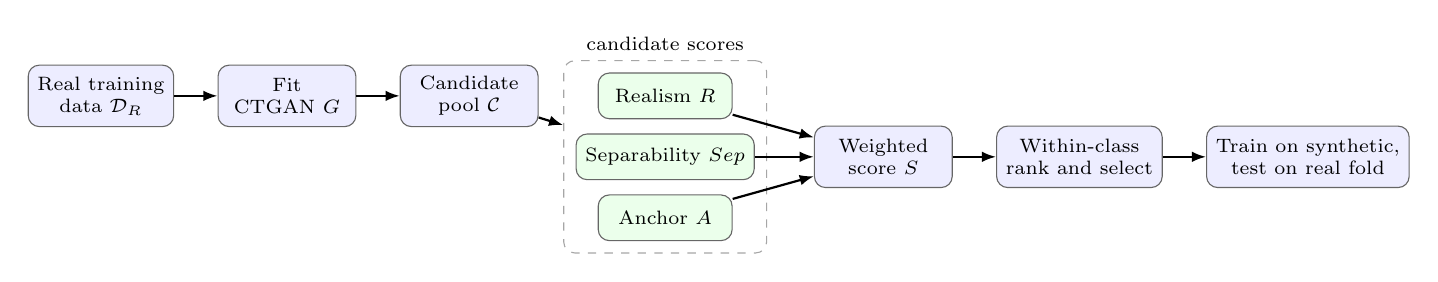
\begin{tikzpicture}[
    node distance=0.55cm,
    block/.style={rectangle, rounded corners, draw=black!60, fill=blue!7,
        minimum width=1.75cm, minimum height=0.78cm, align=center, font=\scriptsize},
    score/.style={rectangle, rounded corners, draw=black!60, fill=green!8,
        minimum width=1.70cm, minimum height=0.58cm, align=center, font=\scriptsize},
    arrow/.style={-{Latex[length=1.8mm]}, thick},
    group/.style={rectangle, rounded corners, draw=black!35, dashed, inner sep=0.15cm}
]
\node[block] (real) {Real training\\data $\mathcal{D}_R$};
\node[block, right=of real] (ctgan) {Fit\\CTGAN $G$};
\node[block, right=of ctgan] (pool) {Candidate\\pool $\mathcal{C}$};

\node[score, right=0.75cm of pool] (realism) {Realism $R$};
\node[score, below=0.18cm of realism] (sep) {Separability $Sep$};
\node[score, below=0.18cm of sep] (anchor) {Anchor $A$};
\node[group, fit=(realism)(sep)(anchor), label={[font=\scriptsize]above:candidate scores}] (scores) {};

\node[block, right=0.75cm of sep] (final) {Weighted\\score $S$};
\node[block, right=of final] (select) {Within-class\\rank and select};
\node[block, right=of select] (eval) {Train on synthetic,\\test on real fold};

\draw[arrow] (real) -- (ctgan);
\draw[arrow] (ctgan) -- (pool);
\draw[arrow] (pool) -- (scores);
\draw[arrow] (realism) -- (final);
\draw[arrow] (sep) -- (final);
\draw[arrow] (anchor) -- (final);
\draw[arrow] (final) -- (select);
\draw[arrow] (select) -- (eval);
\end{tikzpicture}%
}
\caption{\sepa{} post-generation selection pipeline: every operation is fitted or computed using the real training portion of a cross-validation fold; the held-out real fold is used only for evaluation.}
\label{fig:sepaware_pipeline}
\end{figure}

\subsection{Fidelity, Separability, and Privacy Proxies}
\label{sec:proxies}

Fidelity combines numerical-distribution similarity, categorical-proportion similarity, and correlation preservation into a single composite score. Separability is reported using cosine silhouette, a one-nearest-neighbor label-agreement index (SI), and hypothesis margin (HM). These are descriptive geometric measures: higher separation is not automatically clinically desirable, and we do not treat it as such (Section~\ref{sec:discussion}).

The strengthened experiment measures held-out-real minority coverage as the mean distance from each positive test record to its nearest synthetic minority record after training-fold standardization. Minority diversity is the mean pairwise standardized distance among up to 1000 selected minority records. Exact overlap is the proportion of synthetic records with zero distance to a real training record. The membership proxy compares each real training and held-out record's distance to the nearest synthetic record and reports attack \alex{why use the word ``attack'' here?} AUROC. These are empirical diagnostics, not evidence of anonymity or a formal guarantee.

\subsection{Domain-anchored Causal Plausibility Filtering}
\label{sec:dacpf}

\dacpf{} \alex{It is necessary to define the acronym!} generates minority-class CTGAN candidates and ranks their consistency with real minority distributions for domain anchors. The completed COVID-19 experiment compares no augmentation, standard CTGAN augmentation, age filtering, disease-anchor filtering, and combined filtering, evaluated as real-plus-synthetic augmentation (\rsr{}) rather than standalone synthetic substitution. We emphasise that \dacpf{} is a plausibility filter, not causal discovery or effect estimation: ``causal'' describes the clinical origin of the anchor hypotheses, not a claim that the filtering step identifies a causal effect.

\subsection{Replicated $2^2$ factorial experiment}
\label{sec:factorial}

\alex{Would be interesting to add a paragraph to describe the type of factorial experiments beyond the title of this section and, hence, to add some referentes!}

Let $A \in \{-1,+1\}$ encode separability pressure and $B \in \{-1,+1\}$ anchor pressure. The fold-level response is the classifier-averaged \tstr{} Macro-F1,
\begin{equation}
y_{ijk} = \mu + q_A A_i + q_B B_j + q_{AB} A_i B_j + \gamma_k + \varepsilon_{ijk},
\label{eq:blocked}
\end{equation}

\alex{The equation is bit confusing, we should define each variable for factorial model equation, for example, we need to explain what is $i$, $j$, $k$, $q_A$, $A_i$, etc...}

where $\gamma_k$ is a fixed fold block. The high-minus-low factorial effects are $2q_A$, $2q_B$, and $2q_{AB}$. Type-II ANOVA partitions sums of squares among factors, interaction, fold, and residual error; the primary variation percentages exclude the fold block from the denominator so that factor contributions are compared against experimental error rather than against total variation. An unblocked $2^2r$ decomposition that treats folds as replications is also reported in the supplementary material for comparison, but Equation~\ref{eq:blocked} is the more defensible model for paired cross-validation conditions and is used for all primary conclusions.

Both raw and log-transformed responses are analysed. Residual normality is assessed using Shapiro--Wilk and Jarque--Bera tests \alex{include references!}, constant variance is assessed with median-centred Levene (Brown--Forsythe) \alex{include references!}, Fligner--Killeen \alex{include references!}, and Breusch--Pagan tests \alex{include references!}; Durbin--Watson and lag-one Ljung--Box statistics diagnose ordering-related serial patterns but cannot themselves establish independence \alex{include references!}. As noted in Section~\ref{sec:preprocessing}, five-fold training sets overlap by 75\% and the four conditions within a fold are paired, so inference from this design is treated as exploratory rather than as a formal, independently replicated hypothesis test (Section~\ref{sec:stat-limitations}).

\subsection{Strengthened Augmentation Experiment}
\label{sec:strengthened}

The augmentation experiment uses three repeated five-fold stratified partitions and compares real-only training, random oversampling, random undersampling, SMOTE, class-weighted training, standard CTGAN, \sepa{} CTGAN, standard TVAE, and \sepa{} TVAE. Synthetic conditions add positive candidates until the real training fold is balanced, the held-out fold retains its natural prevalence. All missing-value imputation is fitted on the real training fold before resampling or generation. The \sepa{} augmentation score uses realism plus separability with a fixed unit separability weight, no held-out outcome is used to tune the setting.

Logistic regression supplies a linear and calibration-sensitive reference, random forest supplies a nonlinear ensemble, and CatBoost supplies a strong tabular learner. Hyperparameters and the 0.5 classification threshold are held fixed across methods. Fold-level results are retained so generator comparisons can be paired within dataset, repeat \alex{Wouldn't it be better to use ``replications''??}, fold, and classifier. The current manuscript run uses three independently shuffled five-fold partitions with independent fold-specific generator seeds. These repetitions improve stability assessment but remain internal repetitions of the same two dataset samples rather than external validation.

\subsection{Controlled Prevalence-by-overlap Experiment}
\label{sec:controlled}

A separate mechanism experiment varies class prevalence and overlap independently and is not counted as a third health dataset. We generated 2000-record, 15-feature binary-classification problems with 8 informative features, 3 redundant features, 2 clusters per class, and 2\% label noise. Prevalence was set to 5\%, 15\%, or 30\%, and the class separation to 0.4, 1.0, or 2.0, corresponding respectively to high, moderate, and low overlap. Each of the 9 cells used 10 independent data seeds and a stratified 70/30 train-test split.

The comparison includes real-only training, random oversampling, SMOTE, and a SepAware-SMOTE condition. For the latter, SMOTE generates five times the number of required minority candidates, the selector ranks them by nearest-real realism, nearest-hit/nearest-miss margin, and random-forest label confidence, then selects enough records to balance the training data. Logistic regression and random forest are evaluated with AUPRC, Macro-F1, and minority F1 \alex{As previously mentioned, we need to check the term ``minority''.}. A heteroscedasticity-robust linear model tests method-by-overlap and method-by-prevalence interactions.

\subsection{Ethical considerations}
\label{sec:ethics}

The Vigitel analysis uses a secondary survey extract and the COVID-19 analysis uses a de-identified institutional dataset supplied for the qualification research. The manuscript does not infer a new ethics approval number or consent determination. The authors must insert the applicable institutional review board or ethics committee name, protocol identifier, consent or waiver determination, and any access restrictions before submission.

\subsection{Reproducibility}
\label{sec:reproducibility-methods}

The strengthened experiment was executed with Python 3.12, NumPy 1.26.4, pandas 2.2.2, scikit-learn 1.6.1, SDV 1.17.2, CatBoost 1.2.10, XGBoost 3.2.0, imbalanced-learn 0.12.3, and statsmodels 0.14.2. A project-local environment pins NumPy 1.26.4 because the available compiled scientific extensions were incompatible with NumPy 2. Full software-stack notes, executed-notebook identifiers, and artefact-status decisions are given in the code and data availability statement and in Appendix \ref{app:audit}.

\section{Results}
\label{sec:results}

\subsection{Dataset and protocol overview}

The common benchmark included four outcome tasks from three sources. Vigitel obesity and current smoking share the Vigitel source and are not independent cohorts. The analytic samples contained 851 of 5,000 positive obesity records, 83 deaths among 334 COVID-19 admissions, 616 of 5,000 current smokers, and 267 deaths among 5,000 kidney-cohort patients. Every method used the same held-out real folds within a task. The augmentation export contains 1,620 fold--classifier rows (4 tasks, 9 methods, 3 classifiers, 3 repetitions, and 5 folds); no result was aggregated before export.

\subsection{Real-only and conventional imbalance baselines}

Table~\ref{tab:common-benchmark} reports the full augmentation comparison. Real-only training had the highest mean AUPRC for Vigitel obesity (0.287), Vigitel smoking (0.300), and kidney mortality (0.122). Random oversampling had the highest COVID-19 AUPRC (0.355). Threshold-dependent conclusions differed: for kidney mortality, real-only training had mean positive-class recall below 0.001 at the fixed 0.5 threshold, whereas random undersampling increased recall to 0.617 but increased the Brier score from 0.050 to 0.225. These results show why ranking, classification at a fixed threshold, and calibration are reported separately.

\begin{longtable}{p{.17\textwidth}p{.24\textwidth}rrrrr}
\caption{Common augmentation benchmark. Values are means over 3 repeated 5-fold partitions and 3 classifiers (45 paired fold--classifier observations per method and task). Held-out real folds retain natural prevalence; uncertainty and paired inference are reported separately.}\label{tab:common-benchmark}\\
\toprule
Task & Method & AUPRC & Macro-F1 & Recall & Brier & $n$ \\
\midrule
\endfirsthead
\toprule
Task & Method & AUPRC & Macro-F1 & Recall & Brier & $n$ \\
\midrule
\endhead
COVID-19 & Class weighting & 0.348 & 0.530 & 0.373 & 0.234 & 45 \\
COVID-19 & Random oversampling & 0.355 & 0.538 & 0.374 & 0.231 & 45 \\
COVID-19 & Random undersampling & 0.332 & 0.500 & 0.512 & 0.279 & 45 \\
COVID-19 & Real only & 0.351 & 0.493 & 0.113 & 0.198 & 45 \\
COVID-19 & SMOTE & 0.326 & 0.507 & 0.204 & 0.218 & 45 \\
COVID-19 & SepAware CTGAN & 0.323 & 0.534 & 0.362 & 0.239 & 45 \\
COVID-19 & SepAware TVAE & 0.343 & 0.508 & 0.178 & 0.215 & 45 \\
COVID-19 & Standard CTGAN & 0.311 & 0.521 & 0.355 & 0.240 & 45 \\
COVID-19 & Standard TVAE & 0.350 & 0.510 & 0.183 & 0.214 & 45 \\
Kidney mortality & Class weighting & 0.106 & 0.523 & 0.371 & 0.156 & 45 \\
Kidney mortality & Random oversampling & 0.103 & 0.528 & 0.367 & 0.155 & 45 \\
Kidney mortality & Random undersampling & 0.117 & 0.487 & 0.617 & 0.225 & 45 \\
Kidney mortality & Real only & 0.122 & 0.487 & 0.000 & 0.050 & 45 \\
Kidney mortality & SMOTE & 0.096 & 0.520 & 0.256 & 0.131 & 45 \\
Kidney mortality & SepAware CTGAN & 0.110 & 0.526 & 0.175 & 0.099 & 45 \\
Kidney mortality & SepAware TVAE & 0.103 & 0.508 & 0.054 & 0.065 & 45 \\
Kidney mortality & Standard CTGAN & 0.104 & 0.522 & 0.140 & 0.094 & 45 \\
Kidney mortality & Standard TVAE & 0.103 & 0.503 & 0.042 & 0.062 & 45 \\
Vigitel & Class weighting & 0.284 & 0.572 & 0.476 & 0.201 & 45 \\
Vigitel & Random oversampling & 0.281 & 0.573 & 0.486 & 0.202 & 45 \\
Vigitel & Random undersampling & 0.277 & 0.551 & 0.618 & 0.230 & 45 \\
Vigitel & Real only & 0.287 & 0.462 & 0.009 & 0.134 & 45 \\
Vigitel & SMOTE & 0.233 & 0.503 & 0.204 & 0.176 & 45 \\
Vigitel & SepAware CTGAN & 0.256 & 0.527 & 0.254 & 0.175 & 45 \\
Vigitel & SepAware TVAE & 0.252 & 0.492 & 0.089 & 0.153 & 45 \\
Vigitel & Standard CTGAN & 0.247 & 0.511 & 0.219 & 0.176 & 45 \\
Vigitel & Standard TVAE & 0.253 & 0.494 & 0.096 & 0.153 & 45 \\
Vigitel smoking & Class weighting & 0.295 & 0.574 & 0.452 & 0.165 & 45 \\
Vigitel smoking & Random oversampling & 0.291 & 0.582 & 0.467 & 0.165 & 45 \\
Vigitel smoking & Random undersampling & 0.284 & 0.559 & 0.654 & 0.210 & 45 \\
Vigitel smoking & Real only & 0.300 & 0.500 & 0.036 & 0.099 & 45 \\
Vigitel smoking & SMOTE & 0.229 & 0.541 & 0.192 & 0.134 & 45 \\
Vigitel smoking & SepAware CTGAN & 0.249 & 0.565 & 0.288 & 0.143 & 45 \\
Vigitel smoking & SepAware TVAE & 0.255 & 0.526 & 0.099 & 0.111 & 45 \\
Vigitel smoking & Standard CTGAN & 0.217 & 0.536 & 0.216 & 0.145 & 45 \\
Vigitel smoking & Standard TVAE & 0.253 & 0.523 & 0.095 & 0.111 & 45 \\
\bottomrule
\end{longtable}


\begin{figure}[htbp]
\centering
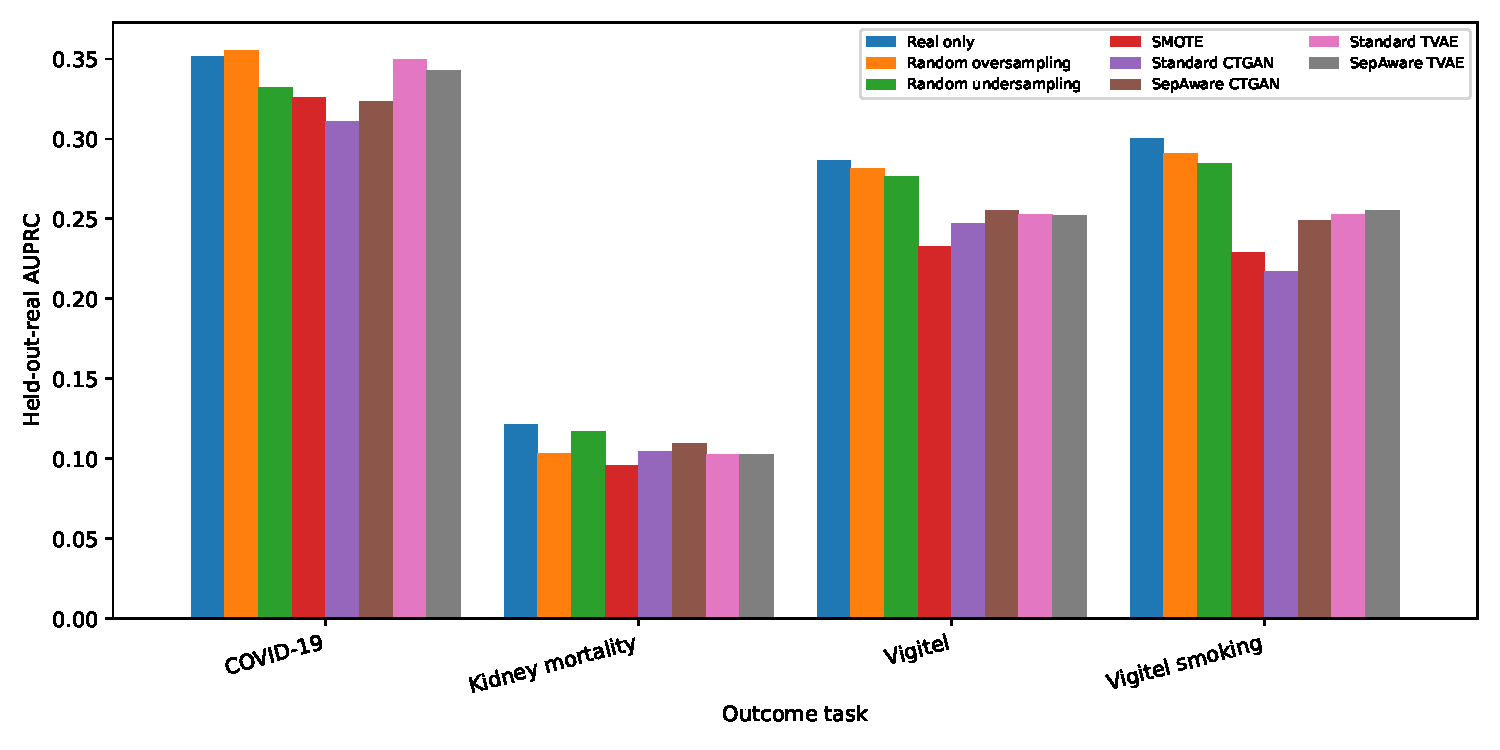
\includegraphics[width=.96\textwidth]{common_benchmark_auprc.pdf}
\caption{Held-out-real AUPRC in the augmentation regime. Bars are means over 3 repeated 5-fold partitions and 3 classifiers. Methods within each task use identical test folds; corrected paired comparisons are shown in Figure~\ref{fig:primary-contrasts}.}
\label{fig:common-auprc}
\end{figure}

\subsection{Standard generators and \sepa{} selection}

For CTGAN, mean AUPRC differences between \sepa{} and standard sampling were 0.012 for COVID-19, 0.009 for Vigitel obesity, 0.031 for Vigitel smoking, and 0.005 for kidney mortality. The Nadeau--Bengio corrected intervals were $[-0.055,0.079]$, $[-0.004,0.021]$, $[0.015,0.048]$, and $[-0.007,0.017]$, respectively. Only smoking remained significant after Holm adjustment ($p_{\mathrm{adj}}=.009$). TVAE differences ranged from $-0.007$ to 0.003, and all corrected intervals included zero. The inferential unit was the mean difference across classifiers within each repeated-CV fold ($n=15$ fold summaries per contrast), not 45 fold--classifier observations.

\begin{figure}[htbp]
\centering
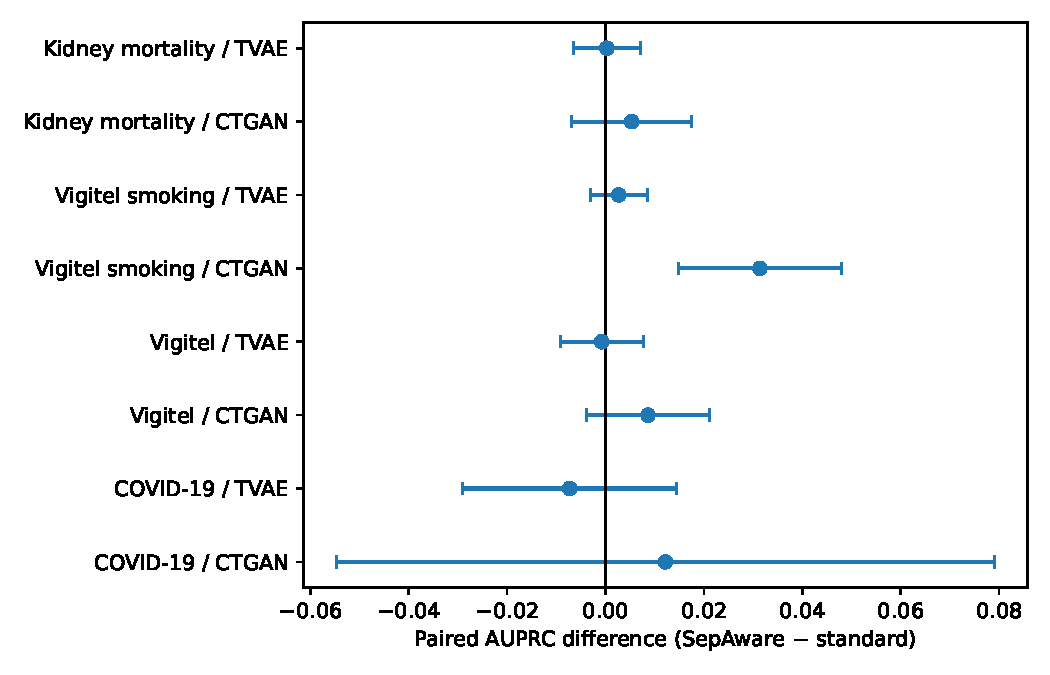
\includegraphics[width=.82\textwidth]{primary_contrasts.pdf}
\caption{Primary paired AUPRC contrasts in real-plus-synthetic augmentation. Points are mean \sepa{} minus standard-generator differences; intervals use the Nadeau--Bengio repeated-cross-validation correction. Eight task--generator tests were adjusted together by Holm's method.}
\label{fig:primary-contrasts}
\end{figure}

The selected CTGAN condition did not surpass the strongest conventional method on any task. Its mean AUPRC was 0.323 for COVID-19, 0.256 for Vigitel obesity, 0.249 for Vigitel smoking, and 0.110 for kidney mortality. The corresponding best conventional values were 0.355, 0.287, 0.300, and 0.122. SepAware therefore improved one generator comparison reliably without establishing superiority over simpler training strategies.

\subsection{TSTR utility}
\label{sec:tstr-results}

The common TSTR experiment trained each classifier only on a synthetic dataset whose class counts matched the corresponding real training fold and evaluated on the untouched real test fold. Standard and selected variants shared candidate pools. Table~\ref{tab:tstr-summary} reports all tasks and both generators; these substitution results are kept separate from augmentation.

\begin{longtable}{p{.20\textwidth}p{.24\textwidth}rrrr}
\caption{TSTR performance. Values are means over 3 repeated 5-fold partitions and 3 classifiers (45 paired observations per condition and task). Synthetic class counts match each real training fold; evaluation uses held-out real records.}\label{tab:tstr-summary}\\
\toprule
Task & Synthetic training data & AUPRC & Macro-F1 & Recall & Brier \\
\midrule
\endfirsthead
\toprule
Task & Synthetic training data & AUPRC & Macro-F1 & Recall & Brier \\
\midrule
\endhead
COVID-19 hospital mortality & SepAware CTGAN & 0.333 & 0.517 & 0.194 & 0.229 \\
COVID-19 hospital mortality & SepAware TVAE & 0.324 & 0.478 & 0.498 & 0.385 \\
COVID-19 hospital mortality & Standard CTGAN & 0.279 & 0.459 & 0.068 & 0.214 \\
COVID-19 hospital mortality & Standard TVAE & 0.332 & 0.491 & 0.468 & 0.347 \\
Kidney-cohort 365-day mortality & SepAware CTGAN & 0.080 & 0.491 & 0.007 & 0.059 \\
Kidney-cohort 365-day mortality & SepAware TVAE & 0.100 & 0.519 & 0.368 & 0.176 \\
Kidney-cohort 365-day mortality & Standard CTGAN & 0.063 & 0.486 & 0.000 & 0.052 \\
Kidney-cohort 365-day mortality & Standard TVAE & 0.102 & 0.524 & 0.336 & 0.160 \\
Vigitel current smoking & SepAware CTGAN & 0.279 & 0.601 & 0.319 & 0.128 \\
Vigitel current smoking & SepAware TVAE & 0.179 & 0.443 & 0.689 & 0.419 \\
Vigitel current smoking & Standard CTGAN & 0.139 & 0.467 & 0.000 & 0.109 \\
Vigitel current smoking & Standard TVAE & 0.183 & 0.428 & 0.700 & 0.432 \\
Vigitel obesity & SepAware CTGAN & 0.279 & 0.548 & 0.175 & 0.148 \\
Vigitel obesity & SepAware TVAE & 0.200 & 0.348 & 0.847 & 0.572 \\
Vigitel obesity & Standard CTGAN & 0.191 & 0.454 & 0.001 & 0.143 \\
Vigitel obesity & Standard TVAE & 0.223 & 0.502 & 0.447 & 0.308 \\
\bottomrule
\end{longtable}


For CTGAN, selection increased mean TSTR AUPRC from 0.279 to 0.333 for COVID-19, 0.191 to 0.279 for Vigitel obesity, 0.139 to 0.279 for smoking, and 0.063 to 0.080 for kidney mortality. TVAE changes were smaller and mixed: 0.332 to 0.324, 0.223 to 0.200, 0.183 to 0.179, and 0.102 to 0.100, respectively. These are descriptive substitution results and do not replace the prespecified augmentation contrasts.

\subsection{Calibration, coverage, diversity, fidelity, and privacy diagnostics}

In augmentation, CTGAN selection reduced positive-class coverage distance for every task: from 4.410 to 4.115 for COVID-19, 1.977 to 1.723 for Vigitel obesity, 3.833 to 3.586 for smoking, and 1.744 to 1.595 for kidney mortality. It also reduced within-positive-class diversity from 11.332 to 7.888, 5.478 to 4.356, 7.340 to 6.310, and 6.827 to 4.425, respectively. Thus closer coverage was consistently accompanied by a more concentrated selected sample.

In augmentation, exact-match rates were zero or below 0.0005, and membership-proxy AUROCs ranged from 0.499 to 0.508 for standard and selected CTGAN. In TSTR, kidney TVAE had much higher exact-match rates: 0.105 for standard TVAE and 0.134 after selection. TSTR detection AUROC was also high for several conditions, reaching 0.995--0.998 for kidney CTGAN and at least 0.979 for kidney TVAE. These results show readily detectable distributional differences and, for kidney TVAE, material duplication risk. Membership-proxy AUROCs remained near 0.5, but none of these measures establishes anonymity. The full marginal similarity, correlation similarity, detection, coverage, diversity, exact-match, and membership-proxy matrix is provided as a machine-readable supplementary table.

\subsection{Dataset-specific anchor and factorial analyses}

Clinical-anchor analyses were not part of the common benchmark. The COVID-19 DACPF experiment required age, cancer, and respiratory-admission variables; comparable anchors were not prespecified for smoking or kidney mortality. Applying invented substitutes after seeing the data would have introduced outcome-guided tuning.

In the five-fold COVID-19 DACPF augmentation run, disease-anchor filtering produced mean Macro-F1 of 0.577 for CatBoost and 0.534 for XGBoost, compared with 0.526 for each classifier under standard CTGAN augmentation. Age-only and combined filters did not improve on standard augmentation. The result is dataset- and classifier-specific.

The blocked $2^2$ anchor-by-separability TSTR analysis was likewise limited to Vigitel obesity and COVID-19. The fold-paired Vigitel separability effect was 0.102 Macro-F1 (95\% CI 0.077--0.128; exploratory $p<.001$). The COVID-19 estimate was $-0.018$ (95\% CI $-0.063$--0.027; $p=.332$). Anchor and interaction intervals included zero for both tasks. Overlapping training folds and shared candidate pools limit these exploratory intervals; they are not independent replications.

\subsection{Controlled simulation}

The simulation varied prevalence and class overlap independently and is not counted as a health-data task. SepAware-SMOTE exceeded ordinary SMOTE in each of nine prevalence--overlap cells for logistic regression, but mean differences were small (0.001--0.024). In pooled heteroscedasticity-robust regression, neither the method contrast nor its overlap and prevalence interactions was distinguishable from zero (all $p>.91$). The simulation therefore supports separating prevalence from overlap but does not locate a stable region in which selection improves predictive performance.

\subsection{Sensitivity and statistical interpretation}

Classifier-by-repetition effects are exported with the primary statistics. Their variation is consistent with the wide corrected intervals for seven of eight primary contrasts. Results from Vigitel obesity and smoking cannot be treated as two independent source replications. The fixed-$\lambda$ grid is retained only as an exploratory development record because configurations were compared on the same folds used for reporting.

\section{Discussion}
\label{sec:discussion}

\subsection{Principal findings}

The study produces two complementary findings. First, the completed synthetic-to-real factorial experiment shows that separability is an attributable, utility-relevant property in Vigitel: enabling separability pressure produces an approximately 0.10 Macro-F1 step, while anchor pressure contributes little. The corresponding COVID-19 attribution is not established because residual fold variation dominates. Second, the strengthened augmentation analysis shows that this large substitution result should not be interpreted as a general augmentation advantage. \sepa{} improves CTGAN AUPRC modestly on both datasets, but random oversampling is highly competitive and \sepa{} does not improve TVAE.

This distinction matters. TSTR asks whether a synthetic dataset can substitute for real training data; augmentation asks whether synthetic minority records add value when the original training records remain available. A method may improve the former without being the best practical solution for the latter. For Vigitel, real-only AUPRC was 0.288, random oversampling achieved 0.284, and \sepa{} CTGAN achieved 0.250. Its advantage was relative to standard CTGAN, not relative to every alternative. For COVID-19, random oversampling achieved the highest mean AUPRC (0.357), while \sepa{} CTGAN and real-only training both achieved 0.354.

\subsection{Comparison with prior work}

The competitiveness of random oversampling agrees with a 2026 JMIR study in which sampling with replacement matched substantially more complex augmentation in small-data settings \citep{huetdastarac2026}. Our results extend that caution to rare outcomes: greater model complexity does not ensure that augmentation adds information. The generator and its sampling mechanism can matter as much as the downstream selector.

Contemporary evaluation frameworks emphasize that fidelity, utility, and privacy can move in different directions \citep{hernandez2025,nanevski2026}. We observe the same pattern within the minority class. \sepa{} CTGAN improves nearest-minority coverage while reducing pairwise minority diversity. A single aggregate fidelity score would not expose that trade-off. The finding also supports calls for explicit privacy and utility threat models rather than duplicate checks alone \citep{kaabachi2025}.

\subsection{When separability helps}

The Vigitel--COVID contrast suggests that separability pressure interacts with the structure and stability of the outcome class. Vigitel provides a larger sample and a more repeatable factorial response. COVID-19 contains only 83 deaths and a heterogeneous set of admission reasons and comorbidities. In that setting, the same scalar margin can be unstable or can compress distinct mortality patterns. The repeated CTGAN augmentation results nevertheless show small positive AUPRC differences for both datasets, suggesting that the selector can improve a candidate pool even when the factorial attribution is weak. This pattern remains exploratory until additional datasets and external or temporal validation test its portability.

The negative TVAE result is equally important. SDV's TVAE does not support native outcome-conditional sampling, so the experiment fitted a minority-conditional feature model. The resulting synthetic minorities had very low diversity, especially for Vigitel. Post-selection could not recover information absent from the candidate pool and sometimes reduced performance further. \sepa{} is therefore not generator agnostic merely because its scoring rule can technically be applied to another generator.

\subsection{The easier-case explanation}
\label{sec:alternative}

Higher separability can represent clearer class-conditional signal, but it can also represent deletion of difficult cases. The strengthened diagnostics support both interpretations. Smaller held-out-minority coverage distance is favorable: selected CTGAN records lie closer to real positive test cases. Lower within-minority diversity is unfavorable: the selector concentrates the candidate distribution. Because no externally validated phenotype labels are available, we cannot determine whether the lost variation is noise, redundant spread, or clinically meaningful heterogeneity.

This trade-off changes the decision rule for the method. A Macro-F1 or AUPRC gain alone is insufficient. A favorable use case requires improvement relative to the corresponding standard generator without material loss of calibration, minority coverage, or clinically meaningful diversity. Boundary-stratified error analysis and expert-defined minority phenotypes are needed to determine how much separability is too much.

\subsection{Privacy implications}

No exact matches were observed and the membership proxy remained near chance. These are reassuring diagnostics but not evidence of anonymity. \sepa{} explicitly prefers records near the real manifold, so the same mechanism that improves utility could increase disclosure risk under a stronger attacker. Membership and attribute inference under explicit attacker knowledge, rarity-stratified analyses, and formal privacy mechanisms remain necessary before any synthetic records are released.

\subsection{Statistical interpretation}
\label{sec:stat-limitations}

The factorial conditions share candidate pools within folds and cross-validation training sets overlap. Blocking captures the paired design, but classical $P$ values remain conditional on one partition, generator configuration, and dataset sample. The strengthened augmentation analysis uses three repeated five-fold partitions with three classifiers; its 45 fold--classifier observations still share source records and do not constitute 45 independent clinical samples. The reported paired intervals are therefore descriptive. Independent datasets and external or temporal validation are required for confirmatory inference.

The appropriate conclusion is therefore conditional. Separability-aware selection controls a property not captured by class balance or global fidelity and can improve CTGAN relative to its unselected candidate pool. It is not uniformly beneficial across generators, it does not consistently beat simple oversampling, and its coverage gains may be purchased with reduced diversity. Those boundary conditions are the scientific contribution of the current two-dataset study.

\section{Limitations}
\label{sec:limitations}

Only two health datasets were available. They differ substantially in size and outcome context, which makes the contrast informative, but two datasets cannot identify a general relationship between intrinsic overlap and SepAware benefit. The current paper should therefore be read as an initial multidataset validation with a controlled mechanism experiment. Additional health datasets with independently observed overlap, prevalence, sample size, and minority heterogeneity are required.

The strongest Vigitel factorial finding comes from one 5000-record sample, one cross-validation partition, one CTGAN configuration, and shared within-fold candidate pools. The strengthened experiment uses three repeated five-fold partitions and 30 training epochs for computational feasibility. Fold-specific generator seeds avoid reusing a single fitted generator, and repeated shuffles measure some partition variability, but all repetitions still reuse the same two source samples. More generator seeds, higher-capacity sensitivity runs, and independent datasets are necessary before formal confirmatory claims.

The fixed lambda grid was exploratory because performance and configuration selection used the same folds. The strengthened analysis fixes the separability weight in advance, but it does not estimate a clinically optimal trade-off between discrimination and minority diversity. The score also depends on a random-forest confidence term; additional boundary models and label-permutation controls are needed to test classifier-specific shortcuts.

The TVAE condition is not directly symmetric with CTGAN. SDV 1.17 does not implement native TVAE conditional sampling, so TVAE was fitted to minority-class features. This is a reproducible conditional-generation strategy, but its low diversity shows that post-selection cannot compensate for a collapsed or highly concentrated candidate pool. A diffusion model and a generator with native conditional support should be added before making a broad generator-agnostic claim.

Minority coverage and diversity are geometric proxies rather than clinically validated phenotype measures. The COVID-19 death class may contain several pathways that are not represented by unsupervised distances. Blinded clinician review and prespecified phenotype or subgroup definitions are required to determine whether removed variation is clinically meaningful. Calibration estimates are also unstable in the small COVID-19 folds.

The privacy analysis is limited to exact matches, nearest-record distances, and a membership proxy. It does not include attribute inference, shadow-model membership attacks, linkage attacks, or a formal differential-privacy guarantee. No synthetic data release should be justified from the present privacy results.

Finally, external or temporal validation is absent. Vigitel spans multiple survey years, but the current evaluation is not a prospective temporal split. The COVID-19 cohort is small and institution-specific. At least one temporal or cross-site evaluation is needed to establish robustness under distribution shift.

These limitations define the next additions to the manuscript: 2--4 further health datasets, repeated partition and generator seeds, a native conditional third generator, expert-informed minority coverage, stronger privacy attacks, and external or temporal validation. If SepAware fails under some of these conditions, those failures should be reported as operational guidance about when separability control should not be used.

\section{Conclusions}
\label{sec:conclusion}

Class imbalance and class overlap are not interchangeable problems. In the synthetic-to-real factorial experiment, explicit separability pressure explains the large Vigitel-obesity utility change but not the COVID-19 variation. In four-task augmentation, SepAware improves CTGAN for COVID-19 and both Vigitel outcomes but not kidney mortality, is inconsistent for TVAE, and is often matched or exceeded by simple rebalancing. Closer minority coverage is accompanied by reduced diversity.

SepAware should therefore be understood as an auditable mechanism for controlling and studying class-conditional geometry, not as a universally superior augmentation method. Its practical use requires evidence that a predictive gain survives simple baselines and does not come from removing difficult but legitimate minority cases. The four-task study establishes this conditional direction and identifies kidney mortality as a clear nonbeneficial boundary case.

\section*{Acknowledgments}

%[AUTHOR TO COMPLETE: acknowledge scientific, technical, institutional, and data-access contributions that do not meet authorship criteria.]

% Generative AI assistance was used during manuscript preparation for drafting, code assistance, and language revision. The authors are responsible for verifying the analyses, citations, interpretation, and final text. This disclosure should be updated to match the exact JMIR submission policy and the authors' final use of AI tools.

\section*{Funding}

% [AUTHOR TO COMPLETE: identify each funder and grant or scholarship number, including support for publication charges, or state that no external funding was received.]

\section*{Conflicts of Interest}

% [AUTHOR TO COMPLETE: disclose financial and nonfinancial conflicts. If none, state ``None declared.'']

\section*{Authors' Contributions}

% [AUTHOR TO COMPLETE after confirming the author list. Assign CRediT roles such as conceptualization, methodology, software, formal analysis, supervision, validation, visualization, and writing.]

\section*{Data Availability}

% Vigitel is a publicly documented Brazilian surveillance system \citep{bernal2017}. [AUTHOR TO COMPLETE: provide the exact access route, extract version, survey years, and terms governing the 5000-record sample.] The COVID-19 hospital-mortality dataset is not distributed with this manuscript. [AUTHOR TO COMPLETE: identify the source institution, access restrictions, and process for qualified access, if permitted.]

% \section*{Code Availability}

% The Overleaf package includes the manuscript source, experiment protocol, strengthened analysis scripts, executed notebook entry point, fold-level results, and figure-generation code. Before submission, the authors should publish a data-safe repository snapshot, add its permanent URL and license here, and confirm that no restricted patient-level records are present.

% \section*{Ethical Considerations}

% [AUTHOR TO COMPLETE: provide the responsible ethics committee or institutional review board, approval or exemption number, consent or waiver determination, deidentification statement, and compensation statement where applicable. These facts cannot be inferred from the local research files.]

% \section*{Software Environment}

% The strengthened experiment used Python 3.12, NumPy 1.26.4, pandas 2.2.2, scikit-learn 1.6.1, SDV 1.17.2, CatBoost 1.2.10, XGBoost 3.2.0, imbalanced-learn 0.12.3, and statsmodels 0.14.2. Generators were run on CPU. The project-local environment pins NumPy 1.26.4 for binary compatibility with the available scientific extensions.


\section*{Abbreviations}
\begin{description}[leftmargin=3cm]
\item[AUPRC] area under the precision-recall curve
\item[AUROC] area under the receiver operating characteristic curve
\item[CTGAN] conditional tabular generative adversarial network
\item[HM] hypothesis margin
\item[SI] separability index
\item[SMOTE] synthetic minority oversampling technique
\item[TSTR] train on synthetic, test on real
\item[TVAE] tabular variational autoencoder
\end{description}

\bibliographystyle{unsrtnat}
\bibliography{references}

\appendix
\section{Reproducibility and Artefact Status}
\label{app:audit}

Table~\ref{tab:audit} lists the status of every research artefact consulted while preparing this paper and states how each was treated. Superseded, protocol-only, or failed runs are excluded from all numerical claims in the main text; only executed, leakage-controlled five-fold notebooks and their exported CSV tables are reported as evidence.

\begin{longtable}{>{\raggedright\arraybackslash}p{.29\textwidth}>{\raggedright\arraybackslash}p{.18\textwidth}>{\raggedright\arraybackslash}p{.45\textwidth}}
\caption{Status of research artefacts consulted during manuscript preparation.}\label{tab:audit}\\
\toprule
Artefact & Status & Manuscript treatment\\
\midrule
\endfirsthead
\toprule
Artefact & Status & Manuscript treatment\\
\midrule
\endhead
Older dataset-specific fixed-$\lambda$ notebooks & Superseded single-split studies & Excluded from numerical claims because they use one 75/25 split.\\
Combined \sepa{} fixed-$\lambda$ notebook & Executed five-fold study & Authority for fold-level fixed-$\lambda$ comparisons (Table~\ref{tab:fixedutility}).\\
Protocol-audited $2^2$ cross-validation notebook & Executed & Superseded by the replicated factorial notebook below; retained only for earlier condition summaries and correlation interpretation during development.\\
Replicated factorial ANOVA notebook (with results) & Latest executed experiment & Authority for the 40 fold responses, ANOVA, effects, and diagnostics (Section~\ref{sec:factorial-results}).\\
Factorial assumption-test script and CSVs & Executed after the notebook above & Authority for expanded residual tests and the blocked-versus-unblocked sensitivity analysis.\\
COVID \dacpf{} raw and summary CSVs & Executed & Authority for augmentation results in Table~\ref{tab:dacpf}.\\
TabPFN augmentation notebook & Failed dependency, no output & Protocol only; no result claimed.\\
Unexecuted causal-filter notebooks & Incomplete protocol & Discussed as development history / future work, not evidence.\\
Cluster-then-augment notebook & No authoritative exported result located & Excluded from numerical results.\\
Strengthened two-dataset augmentation script & Executed three-repeat five-fold experiment & Authority for conventional baselines, CTGAN/TVAE augmentation, calibration, minority coverage/diversity, and privacy-proxy results.\\
Controlled prevalence-by-overlap script & Executed mechanism experiment & Authority for the independent prevalence and overlap manipulation; not counted as a third health dataset.\\
\bottomrule
\end{longtable}

\subsection{Result-authority decisions}

The rerun factorial experiment differs numerically from earlier protocol-audited notes because CTGAN is stochastic even under a fixed, recorded software stack; this paper uses the newly executed observations consistently and does not mix values across reruns. An unblocked $2^2r$ decomposition that treats folds as replications is also present in the repository and assigns COVID-19 90.01\% error and Vigitel 16.92\% error; the main text instead uses the blocked model (Equation~\ref{eq:blocked}), which separates fold variation from treatment variation and yields 81.53\% and 3.59\% respectively (Table~\ref{tab:anova}). Both calculations exist in the repository, but they answer different questions, and only the blocked model is used for the paper's conclusions.

The qualification factorial protocol evaluates standalone synthetic datasets (\tstr{}). The strengthened experiment separately reports real-plus-synthetic augmentation and does not pool the two regimes. AUPRC, calibration, minority geometry, exact-match, and membership-proxy measures are reported only for the strengthened run. Attribute inference, formal privacy guarantees, and external validation remain absent and are reported as limitations rather than estimated after the fact.


\end{document}
